\section{Propuesta}
\subsection{Salas de reunión}
En las salas de reunión se pudo analizar que el tiempo de reverberación no es el mejor para su 
utilización, según la norma DIN$18041$. Por lo que con esta solución se buscará disminuirlo y llevarlo dentro de las tolerancias que indica la norma, 
mejorando así la inteligibilidad y la claridad del habla.

Para esto, pensando también en una solución estéticamente adecuada para las salas, se propone el uso de un "cielo acústico".
Este consiste en un panel de volcanita ranurado ubicado en la parte del techo del recinto como un cielo falso. Para determinar la solución óptima, 
se consideró la distribución del material en el recinto, que cumpliese con los parámetros establecidos, y el costo de la implementación. \\

Es así como se presenta la siguiente propuesta de acondicionamiento:

Para ambas salas de reunión se propone un panel ranurado de volcanita (Rigitone 12/25Q), con un plenum de $200$ mm y aislanglass de $60$ mm en la parte posterior. 
Esto, en el área del cielo en donde se ubica la mesa de las salas. La superficie propuesta en la sala 1 es de $12.5$ $m^2$ y en la sala $2$ de $9$ $m^2$, como se puede observar en las Figuras \ref{fig:propuesta_reunion1} y \ref{fig:propuesta_reunion2}.

\begin{figure}[H]
    \centering
    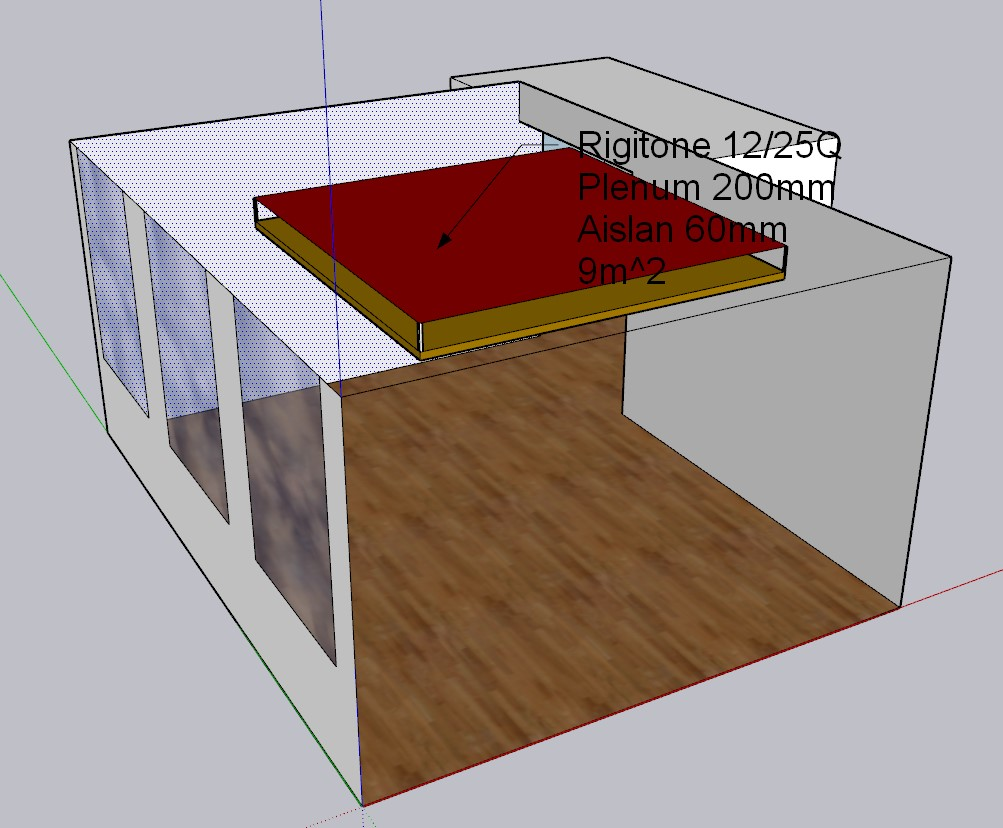
\includegraphics[width=10cm]{Imagenes/Propuesta/propuesta_reunion1.jpg}
    \caption{Propuesta de acondicionamiento en sala de reunión 1}
    \label{fig:propuesta_reunion1}
\end{figure}

\begin{figure}[H]
    \centering
    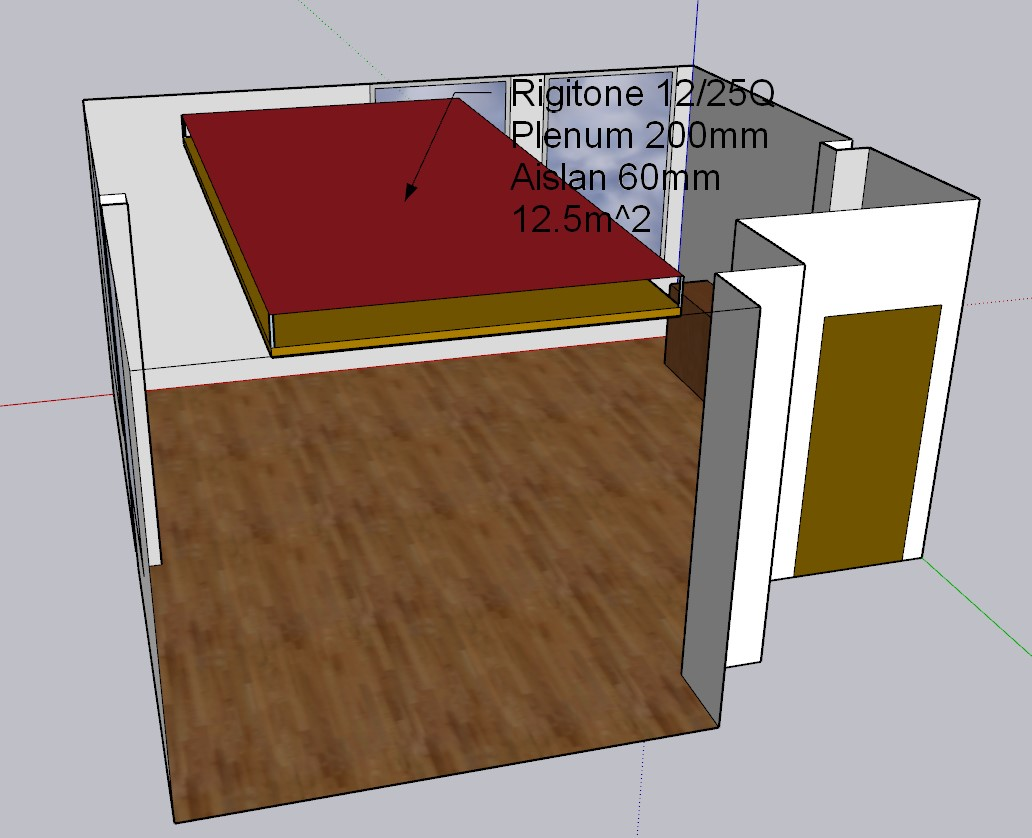
\includegraphics[width=10cm]{Imagenes/Propuesta/propuesta_reunion2.jpg}
    \caption{Propuesta de acondicionamiento en sala de reunión 2}
    \label{fig:propuesta_reunion2}
\end{figure}

El coeficiente de absorción acústica del conjunto de materiales indicados se indican en la tabla \ref{tab: coef abs volcanita Rigitone}
\begin{table}[H]
    \centering
    \begin{tabular}{|lllllll|}
    \hline
    \multicolumn{7}{|c|}{\textbf{Volcanita acústica Rigitone 12/25Q}} \\ \hline
    \multicolumn{1}{|l|}{Plenum} & \multicolumn{6}{c|}{$200$ mm} \\ \hline
    \multicolumn{1}{|l|}{Lana de vidrio} & \multicolumn{6}{c|}{$60$  mm} \\ \hline
    \multicolumn{1}{|l|}{Frecuencia Hz} & \multicolumn{1}{l|}{$125$ Hz} & \multicolumn{1}{l|}{$250$ Hz} & \multicolumn{1}{l|}{$500$ Hz} & \multicolumn{1}{l|}{$1$ KHz} & \multicolumn{1}{l|}{$2$ KHz} & $4$ KHz \\ \hline
    \multicolumn{1}{|l|}{$\alpha$} & \multicolumn{1}{l|}{$0.60$} & \multicolumn{1}{l|}{$0.90$} & \multicolumn{1}{l|}{$0.95$} & \multicolumn{1}{l|}{$0.90$} & \multicolumn{1}{l|}{$0.80$} & $0.75$ \\ \hline
    \end{tabular}
    \caption{Coeficiente de absorción de Volcanita acústica Rigitone}
    \label{tab: coef abs volcanita Rigitone}
\end{table}  

\subsection{Sala de ensayo}
Para la sala de ensayo, se recomienda quitar el material absorbente que se instaló, cambiando así el tiempo de reverberación favorablemente para el uso que le da al recinto.
\begin{figure}[H]
    \centering
    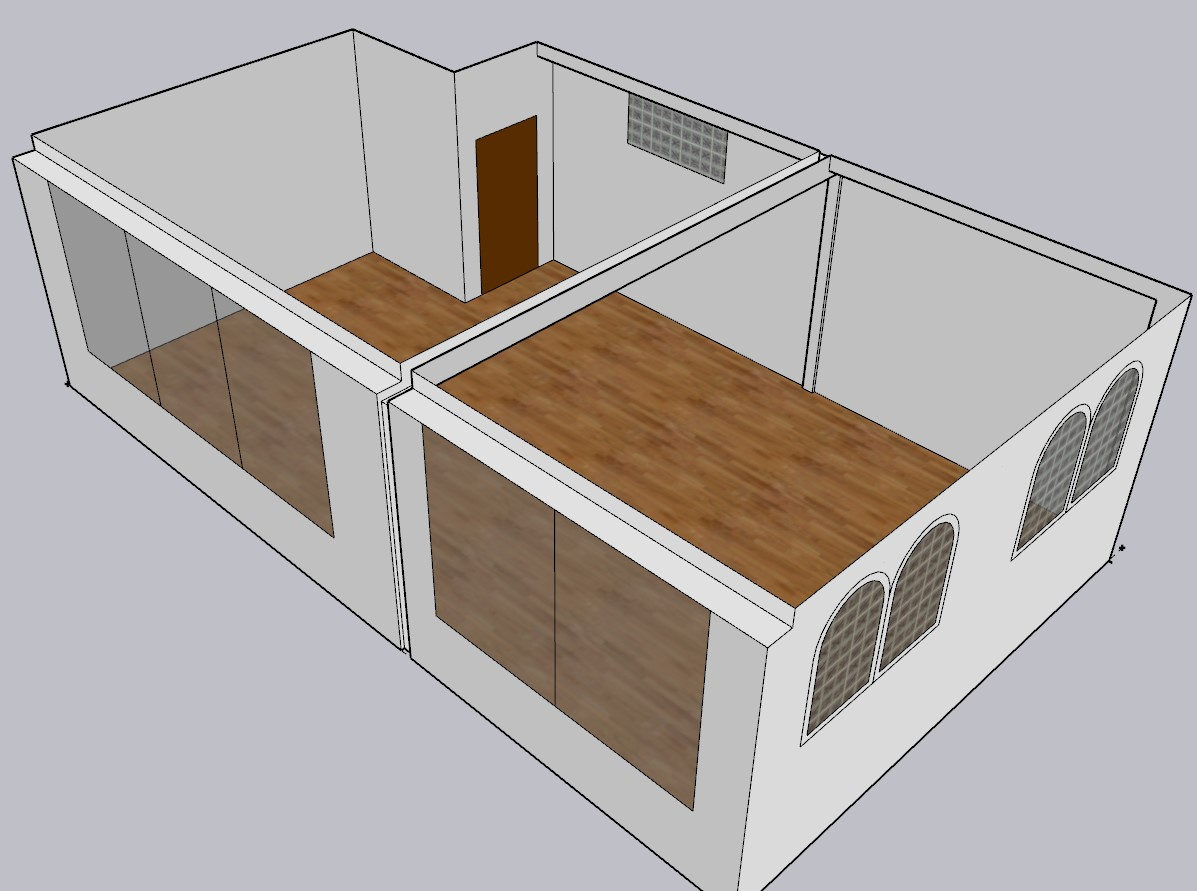
\includegraphics[width=10cm]{Imagenes/Propuesta/Sala ensayo sin paneles.jpg}
    \caption{Propuesta de acondicionamiento en sala de ensayo}
    \label{fig:propuesta_ensayo}
\end{figure}